\documentclass[journal]{IEEEtran}
\usepackage{blindtext}
\let\labelindent\relax
\usepackage[inline]{enumitem}
\usepackage{graphicx}
\usepackage[acronym,toc,shortcuts]{glossaries}
\usepackage{subcaption}
\usepackage{float}

% Abstand nach einer Abbildung verringern
\setlength{\belowcaptionskip}{-5pt}


\usepackage{url}
\usepackage{breakurl}
\def\UrlBreaks{\do\/\do-}

\usepackage[bookmarksopen, bookmarksdepth=2, breaklinks=true]{hyperref}
\usepackage[official]{eurosym}
\usepackage{listings}
\usepackage{multicol}
\usepackage[utf8]{inputenc}  
\usepackage[german]{babel}
% *** GRAPHICS RELATED PACKAGES ***
%
\ifCLASSINFOpdf
\else
\fi


\newacronym{stt}{STT}{Speech to Text}
\newacronym{tts}{TTS}{Text to Speech}
\newacronym{nlu}{NLU}{Natural Language Unterstanding}
\newacronym{nlc}{NLC}{Natural Language Classification}
\newacronym{sdk}{SDK}{Software Development Kit}
\newacronym{cmu}{CMU}{Carnegie Mellon University}
\newacronym{iso}{ISO}{Disk Image Optical}
\newacronym{aws}{AWS}{Amazon Web Services}
\newacronym{ki}{KI}{künstlichen Intelligenz}

\hyphenation{op-tical net-works semi-conduc-tor}

\begin{document}
\title{Speech Triggered Mobility Support And Privacy}

\author{
\begin{center}
  \begin{tabular}{c c c} 
  Jenni Belov & Marius Becherer & Max Wannenmacher \\ 
  Hochschule Furtwangen &  Hochschule Furtwangen &  Hochschule Furtwangen \\ 
  Jenni.Belov@hs-furtwangen.de & Marius.Becherer@hs-furtwangen.de & Max.Wannenmacher@hs-furtwangen.de \\
  \\
  & Michael Zipperle \\ 
  & Hochschule Furtwangen \\ 
  & Michael.Zipperle@hs-furtwangen.de \\
  \end{tabular}
\end{center}}%
       
%\thanks{M. Shell is with the Department
%of Electrical and Computer Engineering, Georgia Institute of Technology, Atlanta,
%GA, 30332 USA e-mail: (see http://www.michaelshell.org/contact.html).}% <-this % stops a space
%\thanks{J. Doe and J. Doe are with Anonymous University.}% <-this % stops a space
%\thanks{Manuscript received April 19, 2005; revised January 11, 2007.}}

% The paper headers
\markboth{Hochschule Furtwangen - Semesterprojekt, Februar 2019}%
{Hochschule Furtwangen - Semesterprojekt, Februar 2019}

% make the title area
\maketitle

\begin{abstract}
%\boldmath 
Aktuelle Sprachassistenten werden von großen IT-Konzernen wie Google, Amazon, Microsoft, Apple oder Baidu angeboten. Die Sprachassistenten umfassen zahlreiche Funktionalitäten, welche i.d.R. zentral in der Cloud von den Anbietern ausgeführt werden. Doch was passiert mit den Eingabedaten der Nutzer? Die Anbieter machen dazu ungenaue Angaben. Die Nutzer können sich nicht sicher sein, ob ihre Privatsphäre und Daten geschützt sind. Es stellt sich die zentrale Forschungsfrage, was mit der sprachbasierten Interaktion zwischen Nutzern und Diensten aktuell geschieht, und welche Konzepte für einen konfigurierbaren Datenschutz durch die Nutzer zukünftig vorstellbar sind. Im Artikel werden die Umfrageergebnisse vorgestellt, die von Sprachassistent-Nutzern im Rahmen dieser Forschungsarbeit ermittelt wurden. Das Ergebnis zeigt insbesondere die Zahlungsbereitschaft für einen individuell konfigurierbaren Datenschutz. Basierend hierauf wird das Konzept für einen konfigurierbaren Sprachassistenten und dessen Architektur präsentiert. Des Weiteren werden Technologien zur zukünftigen Umsetzung dieser Architektur vorgeschlagen.

\end{abstract}

% Note that keywords are not normally used for peerreview papers.
%\begin{IEEEkeywords}
%IEEEtran, journal, \LaTeX, paper, template.
%\end{IEEEkeywords}

% For peerreview papers, this IEEEtran command inserts a page break and
% creates the second title. It will be ignored for other modes.
\IEEEpeerreviewmaketitle


% *** START OF SECTIONS ***--------------------------------------------

\section{Einführung}
Die Sprachsteuerung ist eine Interaktionsmöglichkeit, bei der technische Geräte durch die menschliche Sprache gesteuert werden können. Das nächste Lied, der Wecker oder auch Bestellprozesse können damit initiiert werden.  Die Experten gehen von einem wachsenden Markt für Sprachsteuerungen aus: Die Fachzeitschrift \glqq PR Newswire\grqq{} vermutet, dass Einkäufe über Sprache in den nächsten vier Jahren um das Zwanzigfache ansteigen \cite{prNewswire}. Das Magazin \glqq Campaign\grqq{} schätzt, dass in Zukunft die Suche in Browsern über die Tastatur von der Suche über Sprache ersetzt wird \cite{Campaign}. Die Sprachassistenten beinhalten solche Sprachsteuerungsservices und bilden somit die Schnittstelle zwischen Nutzern und Anwendungen. 

Die Anwendungen eines Sprachassistenten werden Apps genannt und auf einer Plattform in der Cloud ausgeführt. Die Sprachverarbeitung auf der Plattform ist anspruchsvoll, da die Spracheingabe eines Nutzers hochkomplexe Teilprozesse der Sprachverarbeitung durchläuft, bis eine passende Antwort für den Nutzer erzeugt werden kann. Aktuell werden diese Plattformen von großen Cloud-Anbietern angeboten, die über die finanziellen Mittel und das Knowhow jedes einzelnen Teilprozesses verfügen. Universitäten konzentrieren sich i.d.R. auf einen Teilprozess. Sprachassistenten werden von Amazon, Google, Microsoft oder Baidu angeboten, wobei diese viele Funktionalitäten und gute Performance bieten. Jedoch gibt es Bedenken hinsichtlich der Privatsphäre, da aus den Datenschutzerklärungen der Cloud-Anbieter nicht klar hervor geht, was mit den Daten der Nutzer in der Cloud geschieht. Mobile Geräte wie Smartphone und Lautsprecher senden die Spracheingabe eines Nutzers für die Auswertung zum entsprechenden Cloud-Anbieter. Dabei können Daten erfasst und ggf. missbraucht werden. Die Datenverwendung wird in den Nutzungsbestimmungen angegeben, allerdings vermitteln diese eine beschränkte Aussage von den möglichen Verwendungsszenarien, wie das Profiling von Nutzern. 

Aus diesem Grund wurde eine Umfrage mit 110 Teilnehmern durchgeführt. Diese umfasst die Nutzung von Sprachassistenten, die Relevanz des Datenschutzes aus Nutzersicht und  die finanzielle Bereitschaft für mehr Datenschutz. Dabei gaben die Nutzer Anwendungen an, bei denen ihnen Datenschutz besonders wichtig ist. Die Ergebnisse werden im Kapitel \ref{sec:motivaiton} erläutert und stellen die Motivation zur Entwicklung des Konzeptes eines Sprachassistenten mit mehr Privatsphäre für den Nutzer dar. Im Kapitel \ref{sec:konzept} wird ein Konzept vorgestellt durch das Nutzer die volle Kontrolle über ihre Daten erhalten. Zur Erfüllung dieses Konzepts wurde eine Architektur für einen Sprachassistenten entwickelt, welche in Kapitel \ref{sec:architecure} behandelt wird. Anschließend werden in Kapitel \ref{sec:umsetzung} Technologien vorgestellt, mit denen die Architektur umgesetzt werden kann. Eine Beurteilung des Konzeptes, der Technologien und der Umsetzung schließen den Artikel ab. \newline



\section{Related Work}
Sprachassistenten wie Amazon Alexa \cite{alexaAssitent}, Google Assistant \cite{googleAssistant}, Apple Siri \cite{siriAssistent}, Microsoft Cortana \cite{cortanaAssistent} und Baidu DuerOS \cite{baiduAssistant} dominieren aktuell den Markt und sind in Abbildung \ref{fig:sprachassistenten} dargestellt. 

\begin{figure}[!ht]
	\centering
	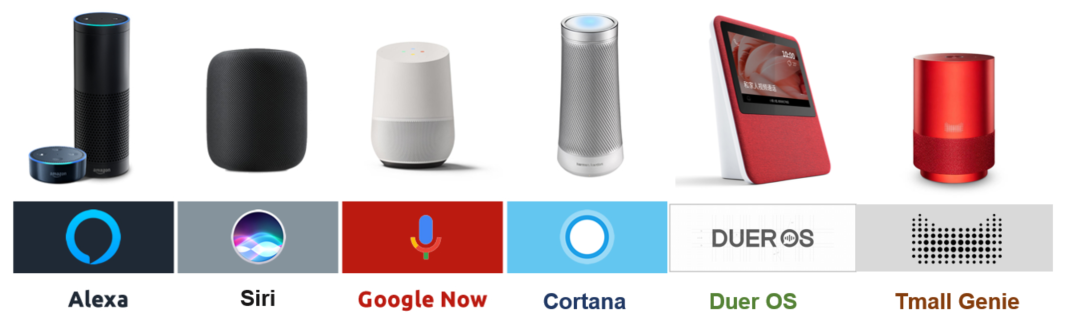
\includegraphics[width=0.9\linewidth]{Picture/Sprachassistenten}
	\caption[Sprachassistenten auf dem Markt\cite{homeAssistants}]{Sprachassistenten auf dem Markt\cite{homeAssistants}}
	\label{fig:sprachassistenten}
\end{figure}

Dabei gehen die Sprachassistenten unterschiedlich mit den Eingabedaten der Nutzer um. Aus den Datenschutzrichtlinien der Anbieter lassen sich keine exakten Informationen finden, was im Detail mit den Eingabedaten eines Nutzers geschieht. Im Folgenden werden die Datenschutzrichtlinien der einzelnen Anbieter kurz beschrieben.

Amazons Alexa verwendet alle Nutzereingaben, um den Sprachservice zu verbessern und personalisierte Werbung anzuzeigen. Eine Beschränkung der Datennutzung für verschiedene Bereiche ist möglich, wodurch sich allerdings auch die Funktionalität einschränkt \cite{alexaPrivacy}.

Google Assistant verwendet die gleichen Berechtigungen, welche für die mobile App des Anbieters gelten \cite{googleShare}. Eine abweichende Einstellung zur mobilen App ist dabei nicht möglich. Die Interaktion mit Google Assistant kann für die personalisierte Werbung genutzt werden, wie sonstige Suchanfragen \cite{googlePrivacy}.

Bei Siri müssen Dienste aktiviert sein, um darauf zurückgreifen zu können. Um die Aussprache und die Funktionalität zu verbessern, werden Daten wie Name, Kontakte, Musik, Suchaktivitäten und weitere Informationen verschlüsselt übertragen. Die Daten werden nicht mit der Apple ID genutzt, sondern mit zufällig erstellter Kennung. Dadurch wird die Privatsphäre für Nutzer gewährleistet \cite{siriPrivacy}.

In den Datenschutzeinstellungen von Microsofts Cortana wird darüber informiert, dass bestimmte Daten \glqq [...] wie z. B. ihre Suchen, Kalender, Kontakte und Orte. [...]\grqq{}\cite{cortanaAssistent} gespeichert werden. Die Datennutzung von Cortana als Personal Assistant ist konfigurierbar. Sind die personalisierten Informationen deaktiviert, kann Cortana nur für Anwendungen wie der Suche und das Festlegen eines Timers genutzt werden. Cortana verwendet personenbezogene Daten nicht für personalisierte Werbung. 

Baidu DuerOS sammelt ebenfalls Nutzerdaten, um die Sprachverarbeitung des Sprachassistenten zu verbessern. Qi Lu verweist auf die vielen Szenarien in denen Baidu Daten sammelt, womit Baidu der Sprung an die Weltspitze im Bereich Künstliche Intelligenz gelingen soll. Die persönlichen Daten eines Nutzers werden übermittelt. Dabei bietet Baidu keine konfigurierbare Privatsphäre an \cite{baiduAI}. 

Seit Februar 2018 gibt es den Sprachassistenten Mycroft Mark II, indem Offenheit und Privatsphäre vereint werden \cite{mycroftsmartspeaker}. Die Funktionalitäten sind hier begrenzt, da der Sprachassistent keine Daten speichert um den Benutzerkontext weiter zu trainieren und zu verstehen.
\section{Motivation}\label{sec:motivaiton}
Zu Beginn wurde durch eine Meinungsumfrage überprüft, ob bei Sprachassistenten mehr Datenschutz gewünscht ist. Dabei haben sich 110 Teilnehmer an der Umfrage beteiligt. Die Teilnehmer umfassten folgende Altersgruppen:
\begin{itemize}
	\item 1 bis 18 Jahre 
	\item 19 bis 25 Jahre
	\item 26 bis 35 Jahre
	\item 36 und älter	
\end{itemize}

55,5 \% der Teilnehmer waren männlich und 45,5\%  weiblich, wie in Abbildung \ref{fig:umfrage_teilnehmer} ersichtlich.

\begin{figure}[!h]
	\centering
	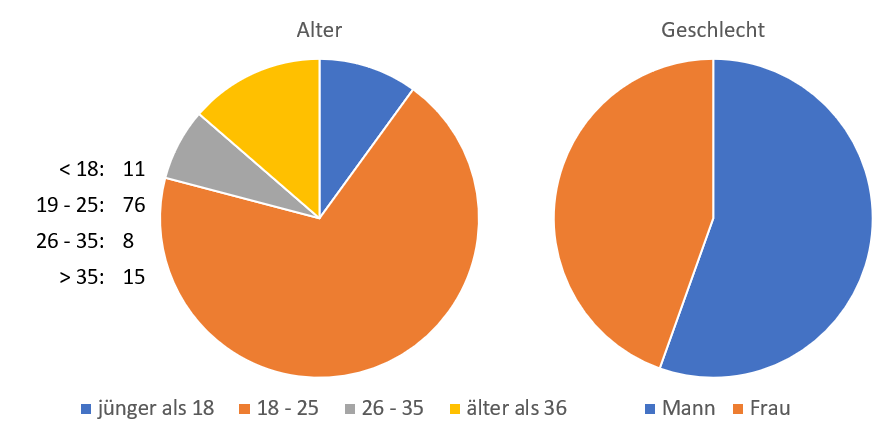
\includegraphics[width=0.9\linewidth]{Picture/umfrage_teilnehmer}
	\caption[Teilnehmer der Umfrage]{Teilnehmer der Umfrage}
	\label{fig:umfrage_teilnehmer}
	
\end{figure}

Den Teilnehmern wurden folgende Fragen gestellt:

\begin{enumerate}	
	\item Wie oft nutzen sie einen Sprachassistenten?
	\item Wissen sie was mit ihren Daten geschieht?
	\item Würden sie Geld für eine hohe Datensicherheit bezahlen?
	\item Wie viel Geld würden sie einmalig für eine hohe Datensicherheit einer Anwendung bezahlen?
	\item Bei welchen Anwendungen ist ihnen Privatsphäre besonders wichtig?	
\end{enumerate}

Bei der ersten Frage stellte sich heraus, dass 44,5\% einmal im Monat oder häufiger einen Sprachassistenten in Anspruch nehmen. In den USA wurde eine Studie von \glqq highervisibility\grqq{} durchgeführt, bei der mehr als 70\% der Teilnehmer einen Sprachassistenten mehr als einmal im Monat verwenden \cite{highervisibility}.
Ein direkter Vergleich der Umfrage mit der Studie aus der USA ist in Abbildung \ref{fig:umfrage_haeufigkeit} zu sehen.

\begin{figure}[!h]
	\centering
	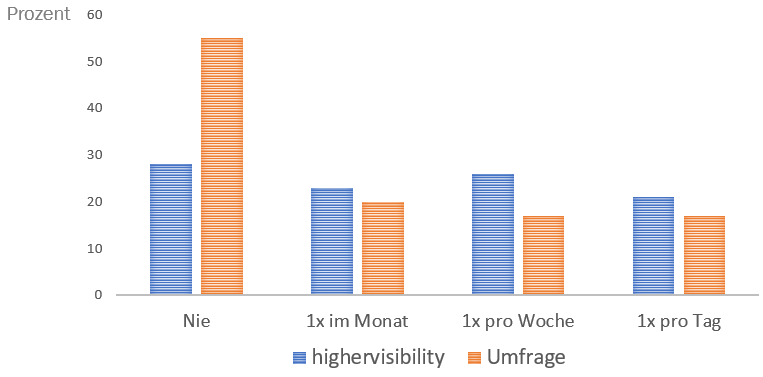
\includegraphics[width=0.9\linewidth]{Picture/umfrage_haeufigkeit}
	\caption[Nutzungshäufigkeit von Sprachassistenten]{Nutzungshäufigkeit von Sprachassistenten}
	\label{fig:umfrage_haeufigkeit}
\end{figure}

In der Studie wurden Menschen aus verschiedenen Altersgruppen und Herkunftsländern befragt. Die im Rahmen dieses Artikels durchgeführte Umfrage wurde überwiegend von jungen Leuten beantwortet.

\begin{figure}[!h]
 	\centering
 	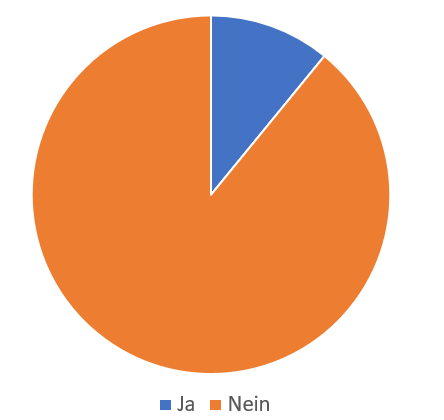
\includegraphics[width=0.5\linewidth]{Picture/umfrage_datenschutz}
 	\caption[Relevanz des Datenschutzes für die Umfrageteilnehmer]{Relevanz des Datenschutzes für die Umfrageteilnehmer}
 	\label{fig:umfrage_datenschutz}
\end{figure}

\newpage

Wie in Abbildung \ref{fig:umfrage_datenschutz} zu sehen ist, wissen 90\% der Teilnehmer nicht, was mit ihren Daten passiert. Die Zahlungsbereitschaft für Datensicherheit ist nach Altersgruppen in Abbildung \ref{fig:umfrage_geld_gruppen} visualisiert. Jeder Vierte würde für eine bessere Datensicherheit bezahlen und 56\% der Teilnehmer sind unsicher, ob sie dafür Geld ausgeben würden. Die Altersbetrachtung nach der Zahlungsbereitschaft ist bei der Gruppe unter 18 Jahren am geringsten. Die Schnittmenge der Teilnehmer, welche \glqq Ja\grqq{} oder \glqq Vielleicht\grqq{} angekreuzt haben, steigt mit zunehmendem Alter.

\begin{figure}[!h]
	\centering
	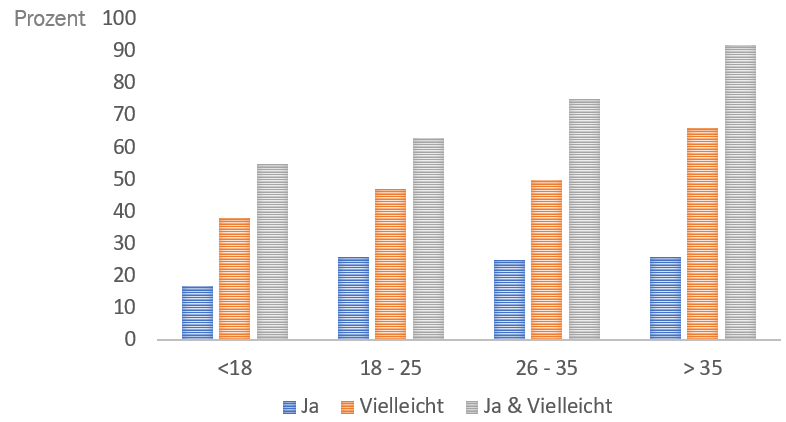
\includegraphics[width=0.9\linewidth]{Picture/umfrage_geld_gruppen}
	\caption[Zahlungsbereitschaft der Teilnehmer in verschiedenen Altersgruppen]{Zahlungsbereitschaft der Teilnehmer in verschiedenen Altersgruppen}
	\label{fig:umfrage_geld_gruppen}
\end{figure}

Der Betrag, welche die Teilnehmer für Anwendungen ausgeben würden variiert sehr und ist in Abbildung \ref{fig:umfrage_betrag} einzusehen. Ungefähr 15\% der befragten Teilnehmer sind nicht bereit dafür zu zahlen, während ein Großteil diese Bereitschaft hat.

\begin{figure}[!h]
	\centering
	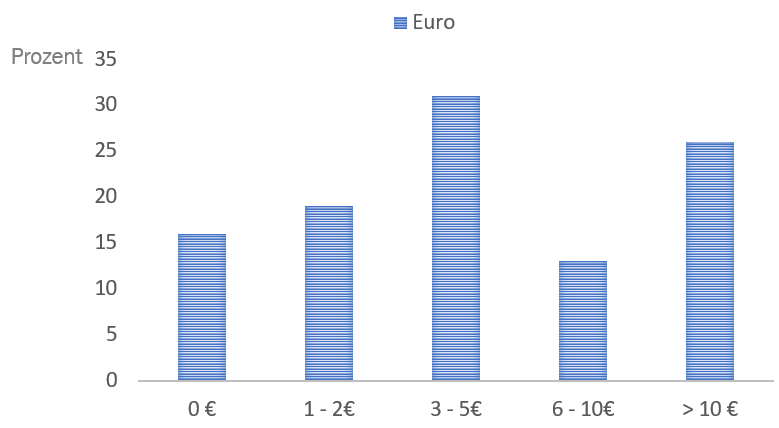
\includegraphics[width=0.9\linewidth]{Picture/umfrage_betrag}
	\caption[Zahlungsbereitschaft der Teilnehmer nach Betrag]{Zahlungsbereitschaft der Teilnehmer nach Betrag}
	\label{fig:umfrage_betrag}
\end{figure}

Wie Abbildung \ref{fig:umfrage_anwendung} zeigt, ist den Teilnehmern die Privatsphäre im Bereich Banking, Haussteuerung, Handysteuerung, Soziale Netzwerke und Chatting besonders wichtig.

Somit lassen sich folgende Schlussfolgerungen aus der Umfrage ziehen:
\begin{itemize}	
	\item Sprachassistenten werden in unterschiedlichem Umfang genutzt
	\item Die Nutzer wissen nicht, was mit ihren Daten geschieht
	\item Nutzer würden für den Schutz ihrer Daten bezahlen
	\item Datenschutz ist in den Bereichen Banking, Chatting, Haussteuerung, Social Media und Handysteuerung wichtig.
\end{itemize}

\begin{figure}[!h]
	\centering
	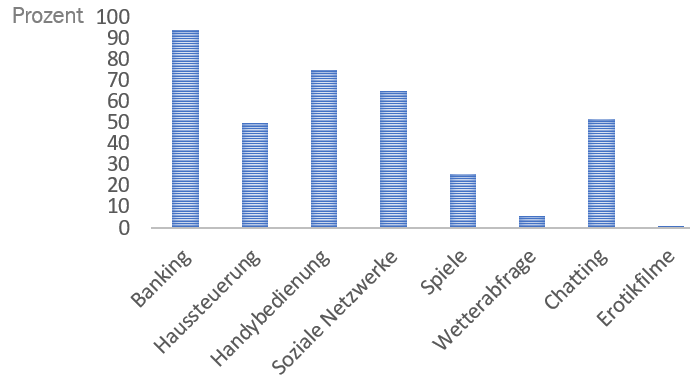
\includegraphics[width=0.9\linewidth]{Picture/umfrage_anwendung}
	\caption[Datenschutzrelevante Anwendungen der Umfrageteilnehmers]{Datenschutzrelevante Anwendungen der Umfrageteilnehmer}
	\label{fig:umfrage_anwendung}
\end{figure}

\section{Konzept}\label{sec:konzept}
Anhand der Umfrage wurde ein Konzept für einen Sprachassistenten entwickelt. Dabei wurden die Kosten für benötigte Ressourcen vernachlässigt. Eine wichtige Anforderung an das Konzept ist der Datenschutz. Die Entwurfsprinzipien für die mehrseitige Sicherheit von Daten nach Kai Rannenberg stellt folgende vier Punkte in den Vordergrund \cite{kairannenberg}:

\begin{enumerate}
	\item Datensparsamkeit
	\item Kontrollmöglichkeiten für den Nutzer 
	\item Auswahlmöglichkeiten und Verhandlungsspielräume 
	\item Dezentralisierung und Verteilung
\end{enumerate} 

Im Rahmen dieses Konzepts erfolgt die Fokussierung auf die ersten drei Punkte. Oftmals erfassen Anwendungen Daten eines Nutzers, die nicht der Verbesserung der Anwendungen dienen, sondern zur Analyse der Nutzer und dem Weiterverkauf verwendet werden. Deshalb soll durch das Konzept sichergestellt werden, dass eine Anwendung nur Daten von Nutzern bezieht, die diese auch tatsächlich benötigen. Des Weiteren sollen die erfassten Daten den Nutzern transparent dargestellt werden. Somit können Nutzer ihre erfassten Daten manipulieren bzw. anonymisieren. 

Daraus ergibt sich für den zu entwickelnden Sprachassistenten folgende Anforderungen:
\begin{itemize}
	\item Nutzergesteuerte Privatsphäre
	\item Funktionalität
	\item Performance
	\item Benutzerfreundlichkeit	
\end{itemize}

Durch die nutzergesteuerte Privatsphäre kann ein Nutzer bestimmen, welche Daten er von sich für bestimmte Anwendungen freigibt. Anwendungen benötigen jedoch zusätzliche Daten eines Nutzers, um dadurch Benutzerfreundlichkeit zu bieten. Ein Beispiel ist die Frage eines Sprachassistenten nach der Wettervorhersage. Weiß der Sprachassistent wo sich ein Nutzer aktuell befindet, so kann dieser die Wettervorhersage für die Position des Nutzer liefern. Sonst müsste der Sprachassistent zuerst den Nutzer fragen, für welchen Ort dieser eine Wettervorhersage wünscht. Will ein Nutzer seine Daten für eine Anwendung nicht freigeben, so kann er einen fiktiven Kontext festlegen. Damit kann der Nutzer diese Anwendung nutzen, jedoch auf Kosten der Benutzerfreundlichkeit.
\section{Architektur}\label{sec:architecure}

\captionsetup[table]{name=Abbildung}
\renewcommand\thetable{8}
\begin{table*}[!ht]
	\centering
	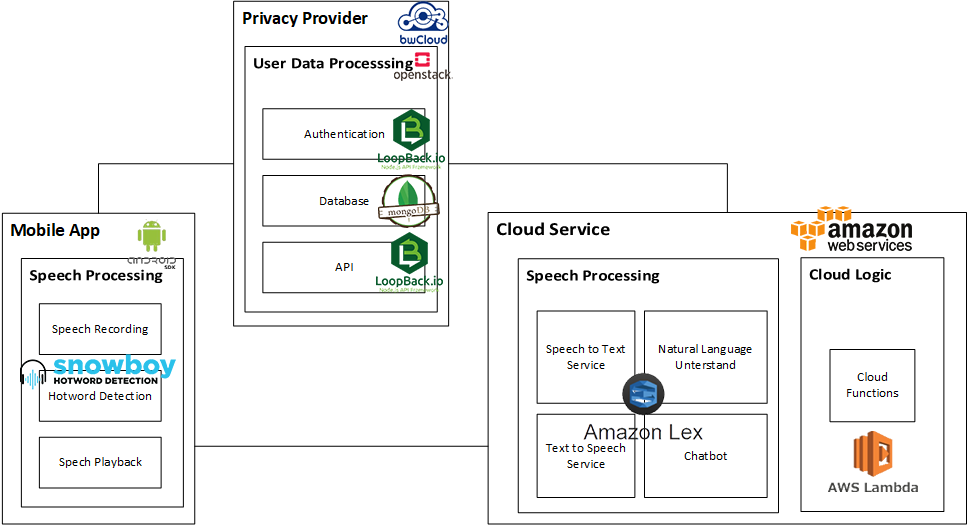
\includegraphics[width=1\linewidth]{Picture/Architektur}
	\caption[Archtiktur Übersicht]{Archtiktur Übersicht}
	\label{fig:architecure}
\end{table*}

Das im letzten Kapitel vorgestellte Konzept wird anhand der in Abbildung \ref{fig:architecure} aufgezeigten Architektur und Technologien umgesetzt. Dabei werden drei Komponenten zur Umsetzung benötigt:
 
\begin{itemize}
    \item Mobile App: Die Mobile App dient als Schnittstelle zum Nutzer. Der Nutzer kann über die App Spracheingaben tätigen sowie sein Profil und Privatsphäre konfigurieren.
    \item Cloud Services: Diese Komponente übernimmt die Sprachverarbeitung und die Erzeugung einer Ausgabe an den Nutzer. Dabei wird zur Erzeugung einer Antwort auf den Privacy Provider zugegriffen.
    \item Privacy Provider: Der Privacy Provider ist das Kernstück, wodurch dem Nutzer mehr Privatsphäre gewährleistet wird. Der genaue Aufbau sowie die Technologieauswahl wird im Folgenden beschrieben. 
\end{itemize}

Für die Kommunikation zwischen mobiler App und der Cloud Services mit dem Privacy Provider wurde eine RESTful \ac{api} ausgewählt. Die \ac{api} basiert auf der RESTful-Technologie, einem Architektur- und Kommunikationsmuster, das häufig bei der Entwicklung von Webdiensten zum Einsatz kommt. Mittels HTTP-Anforderungen wie z.B. GET, PUT-, POST- und DELETE- können Daten ausgetauscht und gespeichert werden \cite{restful-api}. Für die Umsetzung der „Speech Triggered Mobility Support and Privacy“ Anwendung, wurden virtuelle Maschinen, gehostet bei bwCloud, erstellt. Die bwCloud stellt mit Hilfe von OpenStack, \ac{iaas} für Forschung und Lehre in Baden-Württemberg bereit. Sie ermöglicht den Aufbau und Betrieb einer standortübergreifenden Infrastruktur zur Bereitstellung von Computer-Ressourcen \cite{bw-cloud}. Bei Bedarf kann eine bestehende virtuelle Maschine um zusätzliche Ressource erweitert werden, was die Skalierbarkeit des Projektes für zukünftige Anforderungen oder Erweiterungen vereinfacht. Die virtuelle Maschine wird mit Ubuntu Server 18.04.1 LTS betrieben. Mit Hilfe eines 2048Bit RSA Schlüssels kann Verbindung zur virtuellen Maschine hergestellt werden. Für die Umsetzung der REST \ac{api} wurden verschiedene Frameworks betrachtet. 

Loopback ist ein stark erweiterbares, Open-Source Node.js Framework, welches die Entwicklung schneller dynamischer End-to-End REST \ac{api}s ermöglicht. Loopback zeichnet sich durch eine große Community, ausgezeichnete Dokumentation, Vielzahl an Support Möglichkeiten (IBM, StrongLoop) sowie einem breitem Einsatzgebiet aus. Des Weiteren wird es unter anderem auch für kommerzielle Einsatzgebiete, wie z.B. bei der Bank of America, Symantec und der amerikanischen Energiebehörde (Department of Energy) eingesetzt \cite{loopback}.

Loopback ermöglicht es, REST \ac{api}s über ein Command Line Interface Wizard zu erstellen. Es können dynamische Modelle, basierend auf dem gewünschten Datenschema, erstellt werden. Ein weiterer ausschlaggebender Punkt für die Auswahl von Loopback, ist die Unterstützung von Beziehungen unter den erstellten Modellen und der automatischen Erstellung zugehöriger relationaler REST-Endpunkte. Das Framework ermöglicht die Umsetzung einfacher Authentifizierung und Autorisierung durch integrierte rollenbasierte Zugriffskontrollen. Eine Anmeldung von Drittanbietern und OAuth2 ist ebenfalls möglich \cite{mongodb}.

Für die Umsetzung wurde die Loopback Version 3.24.1 verwendet. Das Framework zeichnet sich durch seine Flexibilität aus. Es kann auf einem lokalen Server oder in der Cloud betrieben werden. Ein browserbasierter Explorer ermöglicht Interaktionen mit der \ac{api}. Loopback unterstützt die Anbindung von mehreren Datenspeichern. Für die Umsetzung wurde die Open Source Datenbank MongoDB ausgewählt. MongoDB ist ein verteiltes, flexibles, dokumentbasiertes Datenmodell. Daten werden in JSON-ähnlichen Dokumenten gespeichert. Dies ermöglicht eine Veränderung der Datenstruktur im Laufe der Zeit. Funktionen für Hochverfügbarkeit und Skalierung sowie geografische Verteilung sind einfach durchzuführen \cite{mongodb}. Diese Eigenschaften ermöglichen eine spätere Anpassung oder Verteilung der Infrastruktur.


\section{Umsetzung}\label{sec:umsetzung}
In diesem Kapitel werden Technologien aufgezeigt, mit denen die im letzten Kapitel vorgestellte Architektur umgesetzt werden kann. 

\subsection{Mobile App}
Die Mobile App wird für verschiedene mobile Plattformen wie Android, iOS, Windows Phone und als Webanwendung implementiert. Des Weiteren kann die Mobile App auch in einen Lautsprecher integriert werden. 
\begin{description}
	\item \textit{Speech Recording:} Für das Aufnehmen der Eingabe eines Nutzers ist in den meisten Fällen keine zusätzliche Technologie notwendig. Fast alle mobilen Geräte besitzen bereits ein Mikrofon und die Geräte \acs{sdk} stellt eine Schnittstelle bereit, mit der auf das Mikrofon zugegriffen werden kann.
	\item \textit{Speech Playback:} Auch für das Abspielen eines Streams, kann der eingebaute Lautsprecher über die Geräte \acs{sdk} verwendet werden.
	\item \textit{Hotword Detection:} Im folgenden werden Technologien vorgestellt, mit denen ein Signalwort auf dem mobilen Gerät erkannt werden kann: 
	\begin{itemize}
		\item Snowboy Hotword Detection von Kitt.ai: Snowboy Hotword Detection ist ein Apache lizenziertes Software Projekt zur Erkennung eines Signalwortes. Das Signalwort lässt sich frei bestimmen und das Software Projekt ist optimiert für eingebettete Systeme. Laut dem Hersteller Kitt.ai soll die Hotword Detection unter dem kleinsten Raspberry Pi (single-core 700MHz ARMv6) nur 10\% der CPU
		auslasten \cite{SnowboyHotwordDetection}.
		\item Sensory's TrulyHandsfreeTM: Sensory's TrulyHandsfreeTM ist eine Spracherkennung, die zur Erkennung von einzelnen Wörtern bzw. eines Signalwortes optimiert wurde. Zudem zeigt sie sehr gute Ergebnisse in Umgebungen mit vielen Hintergrundgeräuschen auf. Das Vokabular, welches erkannt werden soll, kann durch Sensory's Grammatik Tool erstellt werden. Sensory's TrulyHandsfreeTM ist verfügbar für Android, iOS, QNX, Windows und Mikrocontroller \cite{TrulyHandsfreeTM}.
		\item Pocketsphinx von \acs{cmu} Sphinx: Sphinx ist ein Forschungsprojekt der \ac{cmu}, das sich mit Spracherkennung befasst. Sphinx basiert auf der Open-Source-Lizenz und kann somit frei verwendet werden, solange erkenntlich gemacht wird, dass es sich um eine Software von \ac{cmu} handelt. Pocketsphinx wurde ebenso wie Sensory's TrulyHandsfreeTM auf die Erkennung von einzelnen Wörter bzw. einem Signalwort optimiert \cite{Pocketsphinx}.
	\end{itemize}
\end{description}

\subsection{Repository}
Das Repository kann durch einen Webserver umgesetzt werden. Dieser Webserver stellt einerseits verschiedene Laufzeitumgebungen und anderseits Apps für den Sprachassistenten zum Download bereit. Die Laufzeitumgebungen können in den folgenden Formaten angeboten werden:
\begin{itemize}
	\item VMWare Image: Das VMWare Image enthält bereits ein vorinstalliertes Betriebssystem sowie alle nötigen Pakete für den Sprachassistenten. Ein Nutzer muss dieses Image in seine VMWare Umgebung (VMWare vSphere, Workstation, Player) importieren und lediglich kleine Netzwerkkonfigurationen vornehmen. Diese Umgebung lässt sich am einfachsten nutzen und benötigt den geringsten Konfigurationsaufwand. Zudem hat der Nutzer die Möglichkeit, die virtuelle Maschine auf einen anderen Server zu übertragen oder Snapshots zu erstellen. Snapshots sind Abbilder einer virtuellen Maschine, die einen bestimmten Zustand widerspiegeln. Dadurch kann bei einer Fehlkonfiguration einfach zum letzten funktionalen Snapshot zurückgesprungen werden \cite{VMWare}.
	\item Docker Image: Das Docker Image ist eine Konfigurationsdatei für eine Container Umgebung. Diese Konfigurationsdatei beinhaltet alle zu installierenden Pakete und Konfigurationen für den Sprachassistenten. Wird diese Konfigurationsdatei in einer Container Umgebung gestartet, werden die Pakete automatisch installiert und der Sprachassistent konfiguriert. Der Nutzer muss lediglich Netzwerkeinstellungen vornehmen, um den Sprachassistenten zu nutzen \cite{Docker}.
	\item \acs{iso}-Image: Das \acs{iso}-Image bietet dem Nutzer die umfangreichste Flexibilität und Konfigurationsmöglichkeit. Der Nutzer kann entscheiden, ob er die Laufzeitumgebung physikalisch oder virtualisiert installieren möchte. Des Weiteren ist diese nicht an eine Virtualisierungssoftware wie VMWare gebunden. Sie kann virtualisiert auf einer privaten oder öffentlichen Cloud installiert werden. Eine öffentliche Cloud nimmt dem Nutzer Aufgaben wie Visualisierung, Backups, Ausfallsicherheit und Load Balancing ab. Mögliche Anbieter sind \ac{aws} mit Amazon EC2 \cite{AWSAmazonEC2}, Microsoft Azure \cite{MicrosoftAzure} und IBM Bluemix \cite{IBMBluemix}. Das \acs{iso} Image beinhaltet auch alle nötigen Pakete für den Sprachassistenten. Der Nutzer wird bei der Installation des \acs{iso} Images durch ein Wizard geführt, bei dem alle Konfigurationen vorgenommen werden.
\end{itemize}

\subsection{Laufzeitumgebung}
\subsubsection{Sprachverarbeitung}
In der Laufzeitumgebung werden Sprachverarbeitungsprozesse durchgeführt. Es gibt zwei Möglichkeiten diese Prozesse durchzuführen, entweder lokal auf der Laufzeitumgebung oder durch die Nutzung von sprach-basierten Cloud Services. Im Folgenden werden die Vor- bzw. Nachteile sowie mögliche Technologien dieser Möglichkeiten erläutert.
\begin{description}
	\item \textit{Cloud-basierte Sprachverarbeitung:} Die Nutzung von sprach-basierter Cloud Services zur Sprachverarbeitung bietet die bestmögliche Performance. Die Sprachverarbeitung basiert i.d.R. auf einer \ac{ki}, welche sich durch Eingabedaten verbessert. Da Cloud Services von vielen Anwendungen genutzt werden, steht der \ac{ki} eine große Anzahl an Eingabedaten zur Verfügung. Dabei ergibt sich als Nachteil, dass die \ac{ki} Eingabedaten eines Nutzers, welche dessen Kontext beschreiben, zur Verbesserung der \ac{ki} genutzt werden und damit die Privatsphäre nicht optimal geschützt ist. Des Weiteren fallen bei der Nutzung von Cloud Services Kosten an. Folgende Anbieter bieten sprach-basierte Cloud Services an:
	\begin{itemize}
		\item \ac{aws}: Amazon bietet zahlreiche sprach-basierte Cloud Services an. Amazon Comprehend ist ein Service für \ac{nlu}, dabei können Einblicke in Zusammenhänge und Beziehungen eines Texte gewonnen werden \cite{AmazonComprehed}. Mit Amazon Translate können Texte, Webseiten und Anwendungen natürlich klingend und akkurat übersetzt werden \cite{AmazonTranslate}. Amazon Transcript kann Sprache zu Text und Amazon Polly Text zu Sprache umwandeln \cite{AmazonTranscript} \cite{AmazonPolly}. Mit Amazon Lex können Konversationsschnittstellen für Anwendungen erzeugt werden. Dabei dient ein Chatbot als Konversationsschnittstelle und kann auf eine bestimmte Eingabe, die zugehörige Antwort erzeugen. Amazon Lex nutzt die gleichen Deep Learning Algorithmen wie der Sprachassistent Alexa von Amazon \cite{AmazonLex}.
		\item Microsoft Azure: Microsoft Azure bietet Cognitive Services an, darunter Services zur Sprache zu Text und Text zu Sprache Konvertierung, Übersetzung von Texten und \ac{nlu}. Des Weiteren wird ein Service zur Sprecher-Erkennung und zur Rechtschreibkorrektur angeboten \cite{MicrosoftAzureCognitiveServices}. Gerade die Sprecher-Erkennung ist ein wichtiger Bestandteil für das in diesem Artikel vorgestellte Konzept eines Sprachassistenten. Durch diesen Service kann ein Nutzer authentifiziert werden.  
		\item IBM Watson: Auch IBM Watson bietet sprach-basierte Cloud Services zur Sprache zu Text und Text zu Sprache Umwandlung an. Des Weiteren wird ein Service für \ac{nlu} und \ac{nlc} angeboten. Durch \ac{nlc} kann die Absicht einer Eingabe ermittelt werden. Mit Watson Assistant kann ein Chatbot realisiert werden \cite{IBMWatsonSpeechServices}.
	\end{itemize}
	\item \textit{Lokale Sprachverarbeitung:} Der Einsatz einer lokalen Sprachverarbeitung auf der Laufzeitumgebung bietet eine bessere Kontrolle der Privatsphäre des Nutzers. Dafür werden auf der Laufzeitumgebung deutlich mehr Ressourcen benötigt und die Performance ist meist schlechter als bei Nutzung der sprach-basierten Cloud Services. Es gibt einige Anbieter, die Frameworks für die lokale Sprachverarbeitung anbieten. Darunter auch Open-Source-Projekte, wodurch für die Nutzung keine Kosten anfallen. 
	\begin{itemize}
		\item Nuance: Nuance arbeitet schon mehr als 25 Jahre an Lösungen für die Sprachverarbeitung und fokussiert sich auf die Integration dieser Lösungen in mobile Geräte wie Smartphones oder Autos. Unter anderem werden Lösungen zur Sprache zu Text und Text zu Sprache Umwandlungen und zur Erstellung eines Chatbots angeboten \cite{Nuance}. 
		\item Mozilla: Mozilla startet mit dem Common-Voice-Projekt eine Initiative, die dabei helfen soll, Maschinen beizubringen, wie echte Menschen sprechen. Diese Initiative befindet sich noch in der Entwicklung. Aktuell werden Datensätze zur Verbesserung der \ac{ki} gesammelt. Dabei gilt die Initiative als Open-Source-Projekt und jede Person kann Datensätze zur Verbesserung hinzufügen. Dazu hat Mozilla eine Webseite und mobile App erstellt mit der Mitwirkende Datensätze prüfen oder Eingabedaten tätigen können \cite{MozillaCommonVoice}. Welches Potential diese Initiative hat, wird sich erst nach der Beendigung der Entwicklung zeigen.
		\item Kaldi: Kaldi ist ein Spracherkennungs-Toolkit, das unter der Apache-Lizenz frei verfügbar ist. Kaldi zielt darauf ab, Software zu liefern, die flexibel und erweiterbar ist \cite{Kaldi}. Das Projekt wird auf GitHub verwaltet und somit können Entwickler zur Verbesserung des Toolkits beitragen.
		\item CMUSphinx: CMUSphinx bietet mit Pocketsphinx eine sprecherunabhängige kontinuierliche Spracherkennung an. Dabei ist Pocketsphinx ein Open-Source-Projekt und wird auf GitHub verwaltet. Pocketsphinx kann in mobilen Geräten eingesetzt werden, dabei wird eine Version für Smartwatches angeboten, die keine Internetverbindung benötigt. Fertige Modelle für die \ac{ki} werden angeboten, es können jedoch auch selbst Modelle trainiert werden \cite{Pocketsphinx}.
	\end{itemize}
\end{description}

\subsubsection{Konfigurationsumgebung}
Die Konfigurationsumgebung kann durch eine Web-Anwendung realisiert werden. Dabei kann der Nutzer über ein beliebiges Gerät mit einem Browser seinen Sprachassistenten konfigurieren. Des Weiteren lassen sich diese Konfigurationen auch mit der Mobilen App vornehmen. Abbildung \ref{fig:prototyp} zeigt einen Prototyp, wie diese Mobile App aussehen könnte. Dabei kann ein Nutzer seinen Kontext einsehen und bestimmen, welche Informationen des Kontexts von Apps genutzt werden dürfen. Der Nutzer kann seinen Kontext manipulieren, falls bestimmte Informationen von einer App benötigt werden; er diese aber aus Gründen der Privatsphäre nicht preisgeben will. Somit hat der Nutzer die volle Kontrolle über seine Daten. 

\begin{figure}[!ht]
	\centering
	\begin{subfigure}{0.32\linewidth}
		\centering
		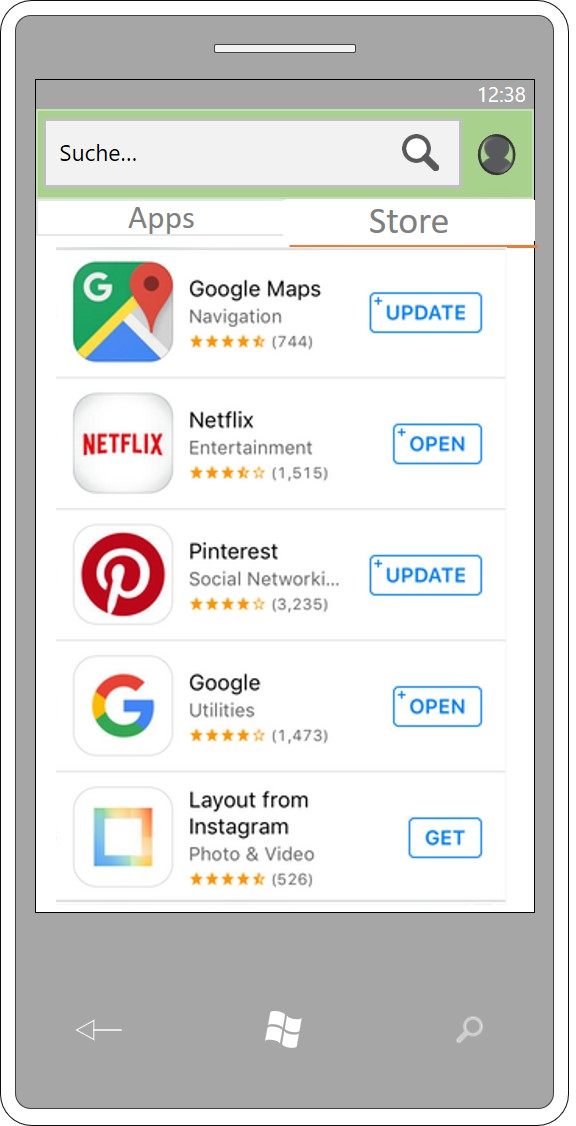
\includegraphics[width=1\linewidth]{Picture/App-Store}
		\caption{Store}
		\label{fig:prototyp1}
	\end{subfigure}%
	\begin{subfigure}{0.32\linewidth}
		\centering
		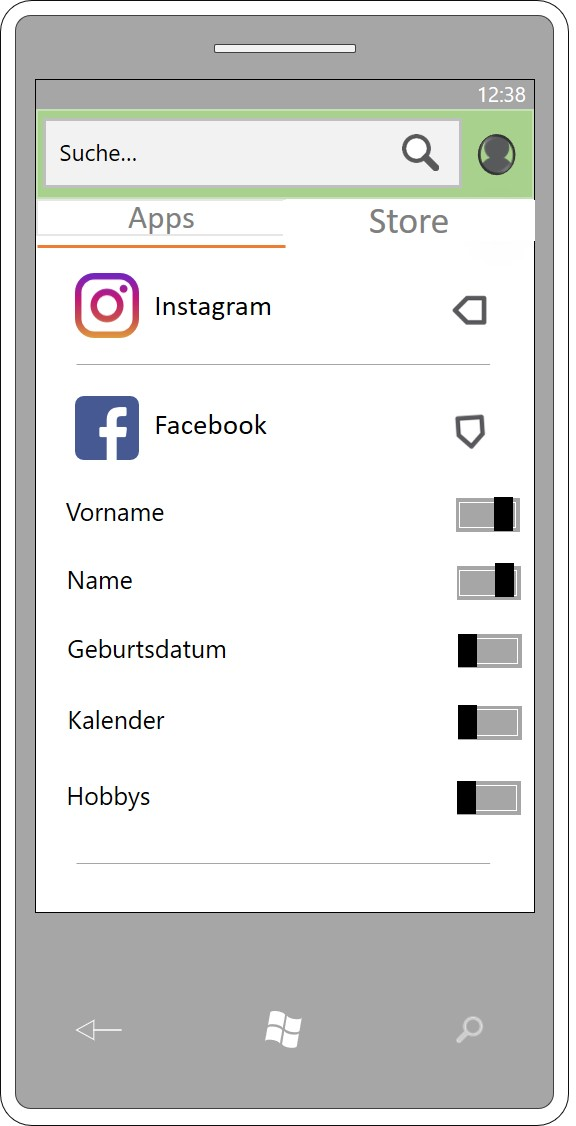
\includegraphics[width=1\linewidth]{Picture/App-Settings}
		\caption{Einstellungen}
		\label{fig:prototyp2}
	\end{subfigure}
	\begin{subfigure}{0.32\linewidth}
		\centering
		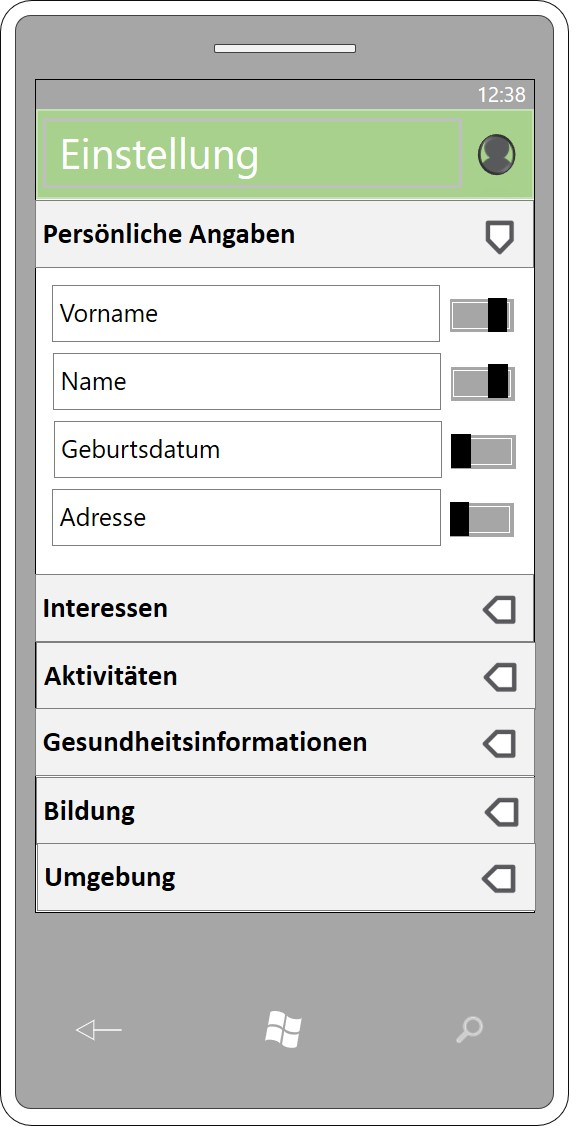
\includegraphics[width=1\linewidth]{Picture/App-Kontext}
		\caption{Nutzer Kontext}
		\label{fig:prototyp3}
	\end{subfigure}%
	\caption{Prototyp der App}
	\label{fig:prototyp}
\end{figure}












\section{Zukünftige Arbeit}
Dieser Artikel zeigt das Problem aktueller Sprachassistenten auf. Mit dem vorgestelltem Konzept kann dem Nutzer eine bessere Privatsphäre gewährleistet werden. Im letzten Kapitel wurden einige Technologien zur Umsetzung dieses Konzeptes vorgestellt. Es zeigte sich, dass es eine große Auswahl an Technologien im Bereich der Sprachverarbeitung gibt. Als nächsten Schritt müssten diese Technologien evaluiert werden, um eine Technologieauswahl treffen zu können. Anhand dieser Auswahl kann festgelegt werden, welche Ressourcen die private Cloud zur Nutzung dieser Technologien benötigt. Des Weiteren lässt sich anhand der benötigten Ressourcen sowie Technologien ein Kostenmodell erstellen. Dieses kann genutzt werden, um eine erneute Umfrage bzw. Interviews mit möglichen Zielgruppen durchzuführen. Die Umfrage soll zeigen, ob die Zielgruppen bereit sind, zusätzliche Kosten für eine bessere Privatsphäre zu bezahlen. Danach kann mit einer prototypischen Entwicklung des Sprachassistenten begonnen werden. Zusätzlich gilt es ein Konzept zu entwickeln, mit welchem Apps auf unerwünschte Datenweitergabe an Dritte geprüft werden können. 
\section{Zusammenfassung}

Durch den entwickelten Prototyp, welcher dem Nutzer Datenschutz und Kontrollmöglichkeiten bietet, konnten einige Rückschlüsse gezogen werden. Dabei konnte die Konzeption bei der Implementierung berücksichtigt werden und Aspekte der mehrseitigen Sicherheit und benutzergesteuerten Privatsphäre finden sich ebenfalls im Prototyp. Der Prototyp besteht aus der Sprachverarbeitungsumgebung (Cloud Services), der Mobile App und dem Privacy Provider.

Anhand der genutzte Cloud Services von Amazon konnten die Funktionalitätsanforderungen erfüllt werden. Aktuell unterstützen die sprachbasierten Cloud Services von Amazon kein Deutsch, deshalb wurde der Prototyp mit Englisch als Sprache umgesetzt. Amazon kündigte jedoch an, bald mehr Sprachen, unter anderem auch Deutsch, anzubieten. Außerdem kann durch die erfüllten DSVGO-Richtlinien der Sprachservices der Datenschutz für die Nutzer gewährleistet werden. Durch die Verwendung der sprachbasierten Cloud Services müssen sich Entwickler nicht detailliert mit der Sprachverarbeitung auseinandersetzen, sondern können auf abstrakter Ebene eine Anwendung entwickeln.  
Bevor ein Nutzer den Sprachassistenten nutzen kann, muss dieser sich authentifizieren. Somit wird der Zugriff vor nichtberechtigten Personen geschützt. In der App können Nutzer verschiedene Profile mit unterschiedlichen Daten anlegen. Hierbei ist die Verwendung von Pseudoprofilen möglich. Im Hinblick auf das Konzept zur mehrschichtigen Sicherheit ist dies wichtig, um Auswahlmöglichkeiten und Verhandlungsspielräume für den Nutzer zu schaffen. Die Nutzerdaten sind in einem Privacy Provider abgelegt. Auch für den Privacy Provider gilt das Konzept der mehrseitigen Sicherheit. Hier ist die Dezentralisierung und Verteilung von großer Bedeutung. Durch die Technologie- und Anbieterauswahl wird auf allen Ebenen der Datenschutz berücksichtigt. Die Daten sind in Deutschland, womit auch eine Rechtslage angewendet wird, die deutlich strenger bei der Datenhaltung ist. Allerdings gibt es beim Privacy Provider auch noch Optimierungspotenzial. Zum einen soll der Ressourcenzugriff konfigurierbarer durch Berechtigung, Dauer und Filterung gestaltet werden. 

In diesem Prototyp wurden nur ein paar Anwendungsfälle umgesetzt. Je nach Nutzer variieren die Anforderungen an einen Sprachassistenten. Verschiedene Anwendungen sollten anhand der Bedürfnisse eines Nutzer aktiviert oder deaktiviert werden können. Dieses Funktionalität könnte den Prototyp in der Zukunft erweitern. Dabei müssen die angebotenen Anwendungen die Nutzer über verwendeten Daten informieren und damit Transparenz  schaffen. Um ein Ökosystem zu schaffen, indem jede Anwendung auf die Daten zugreifen kann, muss ein Standard über die Datenablage geschaffen werden. Andernfalls müssen die Anwendungen die Nutzerdaten selbst verwalten und das Konzept über die Trennung von Daten und Anwendung wäre hinfällig. 

In diesem Artikel wird an verschiedenen Stellen auf das Potenzial von Sprachassistenten verwiesen. Durch die angenehme Bedienung von der Systemintelligenz bietet es einen Mehrwert im Alltag. Allerdings müssen sich verschiedene Branchen öffnen und Schnittstellen anbieten, sodass Buchungen und Reservierungen nicht nur per E-Mail oder Telefon möglich sind. Ist die Infrastruktur von Unternehmen geschaffen, werden Sprachassistenten zusätzlich an Attraktivität für die Nutzer gewinnen.
\section{Danksagung}
Diese Artikel wurde im Rahmen eines Semesterprojekts an der Fachhochschule Furtwangen und unter Betreuung von Prof. Dr. Achim P. Karduck erstellt, dem wir für die gute Betreuung und die vielen Denkanstöße danken.
% *** END OF SECTIONS ***---------------------------------------------


% Can use something like this to put references on a page
% by themselves when using endfloat and the captionsoff option.
\ifCLASSOPTIONcaptionsoff
  \newpage
\fi

\begin{thebibliography}{1}
\bibitem{Campaign}
Christi Olson: "Just say it: The furture of search is voice and personal digital assistant", Campaign 25.04.2016 \url{https://www.campaignlive.co.uk/article/just-say-it-future-search-voice-personal-digital-assistants/1392459},
Zuletzt besucht: 13.07.2018

\bibitem{prNewswire}
OC\&C Strategy Consultants: "Voice Shopping Set to Jump to \$40 Billion By 2022, Rising From \$2 Billion Today", PR Newswire, 28.02.2018, \url{https://www.prnewswire.com/news-releases/voice-shopping-set-to-jump-to-40-billion-by-2022-rising-from-2-billion-today-300605596.html}, 
Zuletzt besucht: 13.07.2018

\bibitem{highervisibility}
Adam Heitzman: "How popular is voice search?", 07.02.2017, higervisibility.com, \url{https://www.highervisibility.com/blog/how-popular-is-voice-search/},
Zuletzt besucht: 13.07.2018

\bibitem{homeAssistants}
”Choosing The Best Voice Assistant For Your Home”, Geeks of Technology,
16.01.2018, \url{https://geeksfl.com/blog/best-voice-assistant/}, Last visit:
20.07.2018 .

\bibitem{kairannenberg}
Rannenberg, Kai. "Mehrseitige Sicherheit—Schutz für Unternehmen und ihre Partner im Internet." Wirtschaftsinformatik 42.6 (2000): 489-497.

\bibitem{cortanaAssistent}
Mircosoft Inc: "Cortana, Ihre persönliche digitale Assistentin", \url{https://privacy.microsoft.com/de-de/windows-10-cortana-and-privacy},
Zuletzt besucht: 05.06.2018

\bibitem{siriAssistent}
Apple Inc.: "Hey Siri, weck mich morgen früh um 7:00 Uhr.",
\url{https://www.apple.com/de/ios/siri/},
Zuletzt besucht: 05.06.2018

\bibitem{alexaAssitent}
Amazon Inc.: "Alexa Assistant"
\url{https://www.amazon.de/b?ie=UTF8&node=12775495031},
Zuletzt besucht: 06.06.2018

\bibitem{alexaPrivacy}
Amazon Inc.: "Alexa Internet Privacy Notice", 23.05.2018,
\url{https://www.alexa.com/help/privacy},
Zuletzt besucht: 06.06.2018

\bibitem{googleAssistant}
Google LLC: "Google Assistant - Just say" ,
\url{https://assistant.google.com/#?modal_active=none},
Zuletzt besucht: 06.06.2018

\bibitem{googlePrivacy}
Google LLC: "Datenschutzerklärung \& Nutzungsbedingungen", 25.05.2018, \url{https://policies.google.com/privacy#whycollect},
Zuletzt besucht: 06.06.2018

\bibitem{baiduAssistant}
Baidu Inc.: "What makes our Artificial Intelligence technology unique"  \url{https://dueros.baidu.com/en/index.html},
Zuletzt besucht: 06.06.2018

\bibitem{baiduPrivacy}
Baidu Inc.: "Baidu Statement of Privacy Protection", \url{http://ir.baidu.com/phoenix.zhtml?c=188488\&p=privacy},
Zuletzt besucht: 06.06.2018


\bibitem{baiduAI}
Jessi hemple: "How Baidu will win china's AI race - and, maybe, the world's", 08.09.2017, \url{https://www.wired.com/story/how-baidu-will-win-chinas-ai-raceand-maybe-the-worlds/},
Zuletzt besucht: 06.06.2018

\bibitem{googleShare}
Google LLC: "Choose what to share with your Google Assistant", \url{https://support.google.com/assistant/answer/7126196?hl=en},
Zuletzt besucht: 06.06.2018

\bibitem{siriPrivacy}
Apple Inc.: "Umgang mit Datenschutz", \url{https://www.apple.com/de/privacy/approach-to-privacy/},
Zuletzt besucht: 06.06.2018

\bibitem{mycroftsmartspeaker}
Jack Wallen: "Mycroft Mark II offers something its digital assistant competitors can't: Privacy and openness", 14.02.2018, \url{https://www.techrepublic.com/article/mycroft-mark-ii-offers-consumers-what-other-digital-assistants-cant-privacy/},
Zuletzt besucht: 06.06.2018	
	
\bibitem{SnowboyHotwordDetection}
Kitt.ai: "Snowboy Hotword Detection",
\url{https://snowboy.kitt.ai/},
Zuletzt besucht: 10.07.2018

\bibitem{TrulyHandsfreeTM}
Sensory: "TrulyHandsfreeTM",
\url{http://www.sensory.com/products/embedded-software-and-sdks/},
Zuletzt besucht: 10.07.2018

\bibitem{VMWare}
"VMWare",
\url{https://www.vmware.com/},
Zuletzt besucht: 11.07.2018

\bibitem{Docker}
"Docker",
\url{https://www.docker.com/},
Zuletzt besucht: 11.07.2018

\bibitem{IBMBluemix}
IBM Bluemix: "Virtual Server",
\url{https://www.ibm.com/cloud/virtual-servers},
Zuletzt besucht: 11.07.2018

\bibitem{AWSAmazonEC2}
Amazon: "Amazon EC2",
\url{https://aws.amazon.com/de/ec2},
Zuletzt besucht: 11.07.2018

\bibitem{MicrosoftAzure}
Microsoft Azure: "Virtual Server",
\url{https://azure.microsoft.com/en-us/services/virtual-machines/},
Zuletzt besucht: 11.07.2018

\bibitem{AmazonComprehed}
Amazon: "Amazon Comprehed",
\url{https://aws.amazon.com/de/comprehend/},
Zuletzt besucht: 11.07.2018

\bibitem{AmazonTranslate}
Amazon: "Amazon Translate",
\url{https://aws.amazon.com/de/translate/},
Zuletzt besucht: 11.07.2018

\bibitem{AmazonTranscript}
Amazon: "Amazon Transcript",
\url{https://aws.amazon.com/de/transcribe/},
Zuletzt besucht: 11.07.2018

\bibitem{AmazonPolly}
Amazon: "Amazon Polly",
\url{https://aws.amazon.com/de/polly/},
Zuletzt besucht: 11.07.2018

\bibitem{AmazonLex}
Amazon: "Amazon Lex",
\url{https://aws.amazon.com/de/lex/},
Zuletzt besucht: 11.07.2018

\bibitem{MicrosoftAzureCognitiveServices}
Microsoft Azure: "Cognitive Services",
\url{https://azure.microsoft.com/en-us/services/cognitive-services/directory/speech/},
Zuletzt besucht: 11.07.2018

\bibitem{IBMWatsonSpeechServices}
IBM Watson: "Speech Services",
\url{https://www.ibm.com/watson/services/},
Zuletzt besucht: 11.07.2018

\bibitem{Nuance}
"Nuance",
\url{https://www.nuance.com},
Zuletzt besucht: 12.07.2018

\bibitem{MozillaCommonVoice}
"Mozilla Common Voice",
\url{https://voice.mozilla.org/de},
Zuletzt besucht: 12.07.2018

\bibitem{Kaldi}
"Kaldi",
\url{http://kaldi-asr.org/},
Zuletzt besucht: 12.07.2018

\bibitem{Pocketsphinx}
CMUSphinx: "Pocketsphinx"
\url{https://cmusphinx.github.io},
Zuletzt besucht: 12.07.2018
\end{thebibliography}

\end{document}


